\chapter{Evaluation}
\section{Evaluate Results}

In the evaluation phase, we respond exhaustively to the company objectives required of us. Since we believe that the goal is very generic, we took the liberty of putting forward a first development model to see if this already satisfies our client's request; A more focused analysis of the business objective is seen by our team as a possible future direction of the project.

\subsection{Assessment of Data Mining Results}
% Summarize assessment results in terms of business success criteria

\begin{figure}%[!h]
\begin{center}
\begin{minipage}{.5\textwidth}
  \centering
  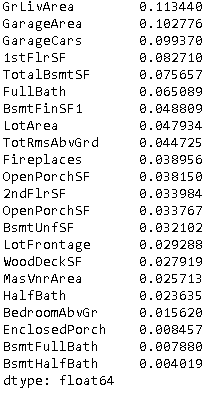
\includegraphics[width=0.7\linewidth]{imgs/feature_scores_numerical.png}
  \captionof{figure}{Feature importance - only numerical}
\end{minipage}%
\begin{minipage}{.5\textwidth}
  \centering
  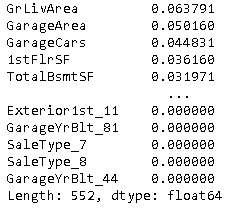
\includegraphics[width=0.7\linewidth]{imgs/feature_scores_categorical.png}
  \captionof{figure}{Feature importance}
  \vspace{50pt}
  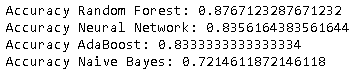
\includegraphics[width=0.7\linewidth]{imgs/accuracy_models.png}
  \captionof{figure}{Accuracy models}
\end{minipage}
\end{center}
\hrulefill\vspace{15pt}\par
\end{figure}

We can answer the following question posed to us:
\\
\emph{What attributes are most related to home price value?}

To answer the question we used the importance of the attributes calculated on the random forest model. It is shown in figure 5.1, for the numerical attributes only, and in figure 5.2 for all the attributes that make up the training set. This calculation is based on the effect that each attribute has on the prediction of the final price; a higher score means that the specific function has a greater effect on the model used to predict a particular variable. 

\subsection{Approved Models}
% After assessing models with respect to business success criteria, the generated models that meet the selected criteria become the approved model

The analysis we have conducted shows that all the models we have developed have a good match in terms of accuracy, as visible in figure 5.2, with the test set. We believe we can predict the price of a home based on its features with reasonable accuracy. 

\begin{figure}[t]
\begin{center}
\begin{minipage}{.5\textwidth}
  \centering
  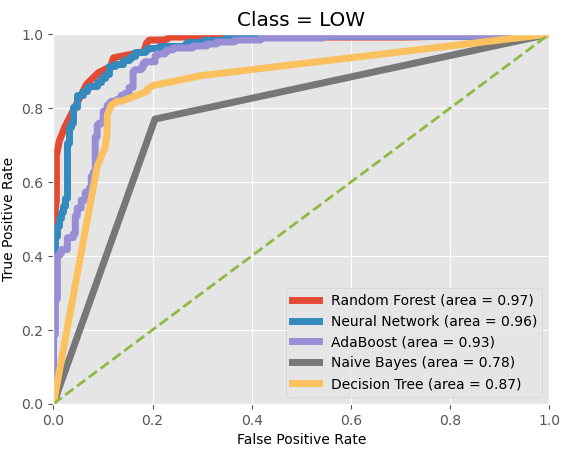
\includegraphics[width=0.9\linewidth]{imgs/roc_low.png}
  \captionof{figure}{ROC Curve Low}
\end{minipage}%
\begin{minipage}{.5\textwidth}
  \centering
  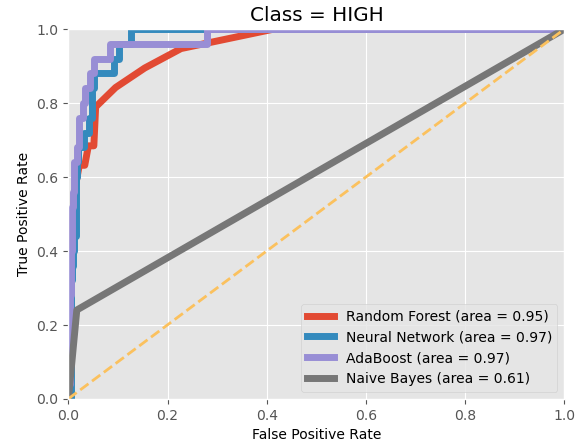
\includegraphics[width=0.9\linewidth]{imgs/roc_high.png}
  \captionof{figure}{ROC Curve High}
\end{minipage}
\end{center}
\end{figure}

\begin{figure}[t]
    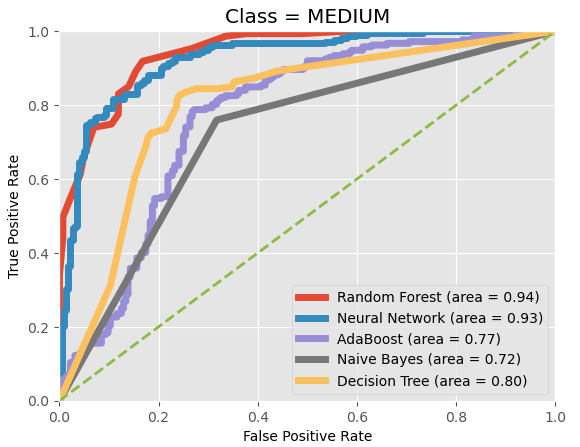
\includegraphics[scale=0.45]{imgs/roc_medium.png}
    \centering
    \caption{ROC Curve Medium}
    \hrulefill\vspace{15pt}\par
\end{figure}

We compared the performance of the models used using different metrics, such as the ROC curve from figure 5.3 to 5.5, which showed a certain score similarity between the Neural Network and the Random Forest model. However, the use of other metrics, such as the confusion matrix, has shed light on the model through accuracy and recall. In conclusion we can say that Random Forest model and Neural Network model are both considered as best machine
learning model for this work. 

\section{Review Process}
% Summarize the process review and highlight activities that have been missed and those that should be repeated

In the project review we checked all the activities carried out so far. Although satisfied with the overall project completed, we continue to ask ourselves whether the analysis carried out to find the most relevant attributes in estimating the price of a house is sufficient or not to start a modernization of the models. However, we believe that a more in-depth analysis, under various profiles, could be the subject of future insights. Regarding the model made, we always ask ourselves the question of whether better accuracy can be achieved. Are we sure we can't do better?

\section{Determine Next Steps}

For the next steps, we have found two that are completely different. One step would allow us to move forward with the software development process, moving to the Deployment phase, while the other step would require a review of the completed phases. In the realization of our software we have followed an incremental model.

\subsection{List of Possible Actions}
% List the potential further actions
\begin{itemize}
    \item Does calculating attribute importance using other models yield the same result?
    \item In the light of what has been discovered, would eliminating the "useless" features lead to an improvement both in terms of model timing, since its dimensionality is reduced, and in terms of performance?
    \item Are we sure these "useless" features don't change over the years? In this case, is still correct removed they to improve our model?
    \item Should we proceed with the deployment?
\end{itemize}

\subsection{Decision}
%  Describe the decision as to how to proceed

To extend the research of the importance of the attributes it is sufficient to use the other models that we have used in the realization of the project. Although these models are not as accurate as the random forest, they could be a valid yardstick with the results obtained.
Removing unnecessary features is a design variant that could make the software grow in terms of quality, however, our team strongly believes that unnecessary parameters will change over the years (for example with the discovery of a material deemed good for construction and subsequently not). However, a hybrid solution of elimination could be adopted, as some parameters tend to never go out of style, such as a large house.
You should talk to the company to understand in which of the two directions they intend to move.